\documentclass{amia}
\usepackage{graphicx}
\usepackage[labelfont=bf]{caption}
\usepackage[superscript,nomove]{cite}
\usepackage{color}
\usepackage{multirow}
\renewcommand*{\thefootnote}{\fnsymbol{footnote}}

\begin{document}

\title{Machine Learning Methods for Discourse Segmentation of Communications in E-Mail Based Behavioral Interventions}

\author{Mehedi Hasan, BS$^{1}$\footnote[1]{Authors provided an equal contribution. \label{footnote1}}, Alexander Kotov, PhD$^{1}$\textsuperscript{\ref{footnote1}}, Sylvie Naar, PhD$^{2}$, Gwen L. Alexander, PhD$^{3}$, April Idalski Carcone, PhD$^{4}$}

\institutes{
$^1$Department of Computer Science, Wayne State University, Detroit, Michigan \\  
$^2$Center for Translational Behavioral Research, Department of Behavioral Sciences and Social Medicine, Florida State University, Tallahassee, Florida\\
$^3$Department of Public Health Sciences, Henry Ford Health System, Detroit, Michigan\\
$^4$Department of Family Medicine and Public Health Sciences, School of Medicine, Wayne State University, Detroit, Michigan\\
}

\maketitle

\noindent{\bf Abstract}
\textit{Communication science approaches to developing effective behavior interventions, such as motivational interviewing (MI), are limited by the traditionally manual qualitative coding of communication exchanges, which is a very resource-intensive and time-consuming process. This study focuses on the analysis of e-Coaching sessions, behavior interventions that are delivered via email and grounded in the principles of MI. A critical step towards automated annotation of e-Coaching communication exchanges is segmentation of emails into textual fragments that correspond to MI behaviors. In this work, we formulate this task as a classification problem and propose lexical, punctuation and part-of-speech features to address it. We experimented both with traditional machine learning method, Conditional Random Field (CRF) and deep learning methods, such as Multilayer Perceptrons (MLPs), Bidirectional Recurrent Neural Networks (BRNNs) and Convolutional Recurrent Neural Networks (CRNNs). Results indicate that CRNN outperformed CRF, MLP and BRNN achieving 0.990 macro F1-score overall and 0.821 macro F1-score for detecting new segment.}

\section*{Introduction}
The emergence of e-Health technologies opened up new ways to deliver a variety of behavioral interventions to any demographic group of patients in any geographical location. Motivational interviewing (MI), an evidence-based communication technique to increase intrinsic motivation and self-efficacy for behavior change\cite{miller2012motivational,miller2009ten,miller2009toward}, is one type of these interventions. MI sessions are generally aimed at eliciting ``change talk'', or statements of intrinsic motivation about patients' own desire, ability, reasons, need for and commitment to behavior change, which have been established by previous research\cite{apodaca2009mechanisms} as a reliable mediator of health behavior change. However, communication science approaches to understanding the efficacy of MI are inherently limited by traditional qualitative coding methods. 

Qualitative coding of motivational interviews with pre-defined codes has been traditionally performed manually by trained annotators, which is a tedious and resource-intensive process that involves several iterations of reading, comprehension and interpretation of interview transcripts. Rapidly developing computational technologies, specifically, machine learning methods, offer a unique opportunity to accelerate this process. In particular, machine learning methods have been successfully applied to a variety of analytical tasks involving textual data, such as classification\cite{nigam2000text} and sentiment analysis\cite{wang2012baselines}. In our previous work, we examined the utility of machine learning methods for automated annotation \cite{hasan2016study,kotov2015interpretable} and analysis \cite{hasan2018predicting} of in-person MI sessions. Specifically, we demonstrated that machine learning methods can be utilized for annotation of MI transcripts according to a simple communication code scheme with the accuracy comparable to human coders\cite{hasan2016study}. Experimental data utilized in these studies, however, were prepared by transcribing audio conversations, which were clearly segmented into utterances by a counselor, a patient and a caregiver. 

In this study, we focus on the analysis of e-Coaching sessions, behavior interventions that are delivered via email and grounded in the principles of motivational interviewing. Specifically, the e-Coaches involved in this study used emails to communicate motivation-enhancing messages that encourage healthy eating among GenY adolescents. e-Coaching data is comprised of email responses, which are free-text documents, unlike more traditional dyadic clinical interviews that are naturally segmented into utterances due to their conversational nature.

The unstructured nature of e-Coaching exchanges poses a unique set of challenges for their qualitative analysis. A significant barrier to fully automating the behavior coding process of e-Coaching emails is their segmentation into textual fragments that correspond to distinct communication behaviors. Automating this task is a unique and challenging problem due to the following major reasons:

\begin{enumerate}
\item Emails are unstructured text that contains informal information exchange in a non-traditional format.
\item Discourse segments in e-Coaching emails do not necessarily correspond to sentences or collection of sentences. One sentence can be segmented into multiple MI behavior fragments. On the other hand, an MI behavior may comprise several sentences.
\end{enumerate}

Figure~\ref{fig:text-segment} illustrates a segmentation of an e-Coaching email exchange, in which the first sentence is segmented into 2 MI behavior fragments, while the fourth and fifth segments correspond to one and three sentences, respectively. Segmentation of e-Coaching emails corresponds to a special type of discourse analysis \cite{webber2012discourse} aimed at better understanding the effective e-Coaching communication strategies and revealing the unique socio-psychological characteristics of a patient.

\begin{figure}[!htb]
    \centering
    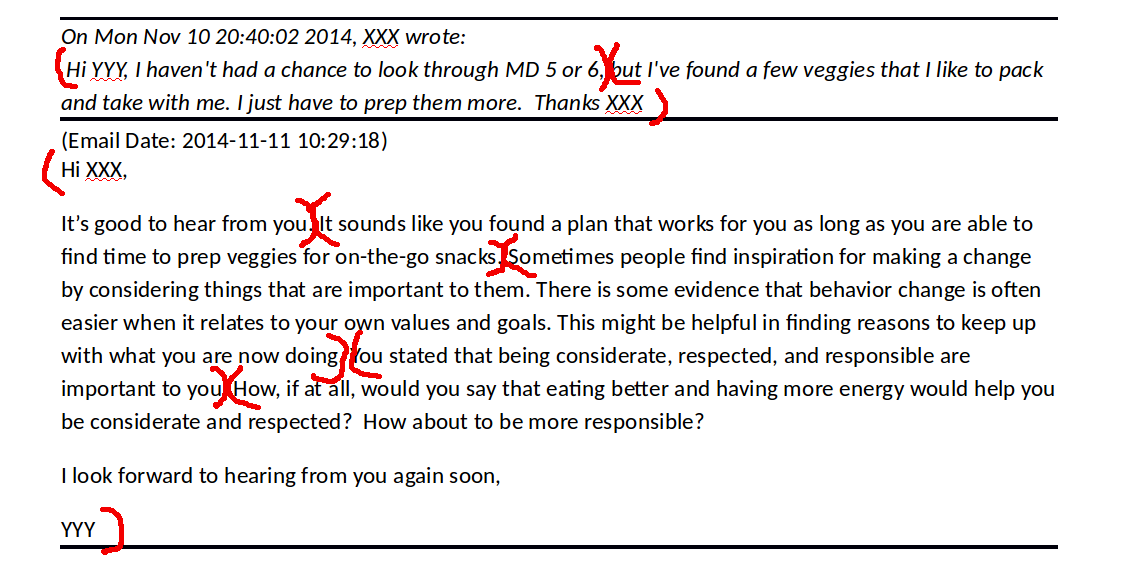
\includegraphics[width=0.9\textwidth]{figures/segment-example.png}
    \caption{\textbf{Example of e-Coaching emails segmented into fragments that correspond to MI behaviors of an e-Coach and a patient}.}
    \label{fig:text-segment}
\end{figure}

The goal of this research study is to assess the applicability of machine learning methods for automated segmentation of e-Coaching emails into textual fragments corresponding to individual behaviors, which is the first step of the coding process of e-Coaching communications. In particular, we introduced lexical, semantic and punctuation features and experimented with both traditional supervised machine learning method, linear-chain Conditional Random Field (CRF) and deep learning methods, such as Multilayer Perceptrons (MLPs), Bidirectional Recurrent Neural Networks (BRNNs) and Convolutional Recurrent Neural Networks (CRNNs), to find the best performing method and feature combination. 

Relevant previous work in the biomedical domain primarily focused on segmentation of text into sections and headers\cite{apostolova2009automatic,denny2009evaluation,tepper2012statistical,cho2002text} or sentence boundary detection\cite{griffis2016quantitative,kreuzthaler2015detection,treviso2016sentence,fraser2015sentence}. Apostolova et al.\cite{apostolova2009automatic} applied SVM along with word-vector cosine similarity metric combined with several heuristics to segment clinical reports into sections, such as demographics, history, procedure, finding and impression. After identification of each line in the document, Tepper et al. \cite{tepper2012statistical} trained Maximum Entropy models for section classification. Denny et al.\cite{denny2009evaluation} proposed a SecTag algorithm, which combined natural language processing techniques, terminology-based rules and Naive Bayes classifier to identify the sections and headers that achieved 99\% recall with 95.6\% precision. On the other hand, SVM based on prosodic and part of speech features \cite{kreuzthaler2015detection} and recurrent convolutional neural networks using word embeddings \cite{griffis2016quantitative} were utilized for detecting sentence boundaries. Segmentation of e-Coaching emails is different from a traditional shallow discourse analysis of conversations \cite{galley2003discourse} in that the focus is on segmentation, rather than on determining the types of transitions between the utterances or assigning utterances to speakers.

Recently, an online clinical intervention called MENU GenY \cite{alexander2017motivations} (Making Effective Nutrition Choices for Generation Y) was proposed and evaluated. MENU GenY is a technology-based public health intervention that relies on personalized e-coaching to encourage increased fruit and vegetable intake among young adults, aged 21-30. The goal of MENU GenY was to develop a better coding dictionary among GenY to improve eating habits. However, segmentation of clinical conversation in the context of electronically delivered interventions, in particular, segmentation of clinical interaction text into groups of MI behaviors, is still performed manually, which slows down qualitative analysis of these interventions. This study introduces a novel computational approach to address this problem and the authors are unaware of any other work that focused on the same problem.  

\section*{Methods}
\subsection*{\textit{Data collection}}
The experimental dataset for this work was constructed from 49 e-coaching sessions, which include a total of 3,138 segmented and annotated MI behaviors. Each session represents an MI intervention delivered via email. We formulate the segmentation task as a binary classification problem where each word annotated with a label 1 or 0, to indicate whether it preceds a new segment or not. We experimented both with traditional machine learning method, linear-chain Conditional Random Field (CRF) and deep learning methods, such as Multilayer Perceptrons (MLPs), Bidirectional Recurrent Neural Networks (BRNNs) and Convolutional Recurrent Neural Networks (CRNNs). For MLP models, e-Coaching email exchanges are partitioned into adjacent word pairs. Each pair is classified into either ``new segment'' or ``same segment'' class. The gold standard is manually segmented where adjacent word pairs are classified into ``new segment'' class. If all adjacent word pairs of a block of text are classified into ``same segment'' class, the entire block is treated as one textual fragment corresponding to a single MI behavior. In total, we obtained 95,421 word pairs, which include 3,138 ``new segment'' and 92,283 ``same segment'' instances. For deep learning models, an email was taken as input sequence, such that PoS tags and word embedding of each word or punctuation marks were used as input and binary labels (1 or 0) corresponding to ``new segment'' and ``same segment'' classification decision were considered as the output of the model at each step. In the gold standard, words within the same segment were assigned the label of 0 and the last word or punctuation mark of a segment were assigned the label of 1.    

\subsection*{\textit{Features}}

We utilized three types of features in conjunction with CRF, MLP, BRNN and CRNN methods: lexical, punctuation and topic features. Lexical features represent each word in a pair as a binary vector, in which 1 corresponds to the word in question and 0 to all other words. Since part-of-speech (PoS) tags \cite{kotov2015interpretable,hashimoto2016topic,lu2016modeling} have been shown to be effective semantic abstractions of individual words, we used topic features for our experiment. Punctuation marks, which correspond to one of the symbols \{`.', `,', `!', `?', `:', `;'\} between a pair of words, are also employed as a feature since punctuation marks designate the boundary of a sentence, clause and phrase and often also correspond to segment boundary.   

\subsection*{\textit{Classifiers}}

We experimented both with traditional classifiers, including Conditional Random Field (CRF) and deep learning models, such as Multilayer Perceptrons (MLPs) Bidirectional Recurrent Neural Networks (BRNNs) and Convolutional Recurrent Neural Networks (CRNNs).

\textbf{Conditional Random Field}: state-of-the-art supervised classification method proven to be effective for text categorization\cite{joachims1998text} for its ability to cope with high dimensional input feature space. SVM finds the hyperplane that maximizes the separation between the closest ``new segment'' and ``same segment'' training examples. We scaled our dataset to utilize linear SVM with optimal cost 512 in experiments.   

\textbf{Deep Learning Methods}: this method considers each training sample as a point in the input feature space. For a new test sample, Euclidean distance is calculated to find the k-nearest classified neighbors from the training set. Finally, the test sample is classified into a majority class of its k-nearest neighbors. We experimentally determined that best performance was achieved when the number of neighbors is 3. 

\textbf{Bidirectional Recurrent Neural Networks}: RNN is a neural network architecture designed to capture sequential patterns. When we predict the new segment point using RNNs, particular combinations of words in a sequence will indicate the change of MI behavior. Long Short Term Memory (LSTM) networks\cite{hochreiter1997long} are a special type of RNN that are capable of handling variable size input sequence and have an internal memory that can be reset. GRU\cite{chung2014empirical} is a variant of LSTM mathematically represented by the following formula:

\textbf{Convolutional Recurrent Neural Networks}: RNN is a neural network architecture designed to capture sequential patterns. When we predict the new segment point using RNNs, particular combinations of words in a sequence will indicate the change of MI behavior. Long Short Term Memory (LSTM) networks\cite{hochreiter1997long} are a special type of RNN that are capable of handling variable size input sequence and have an internal memory that can be reset. GRU\cite{chung2014empirical} is a variant of LSTM mathematically represented by the following formula:

\begin{figure}[!htb]
    \centering
    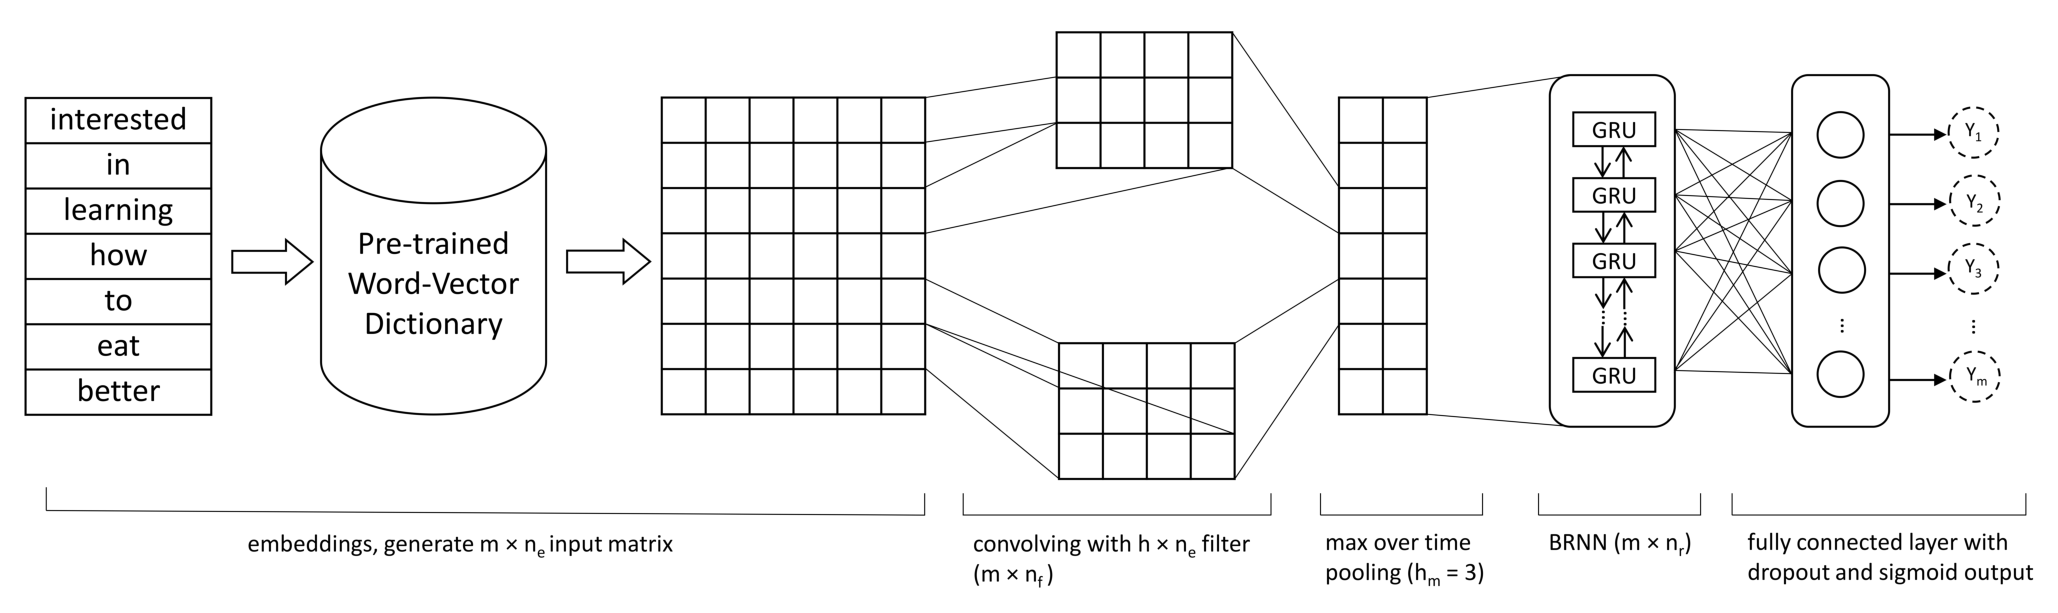
\includegraphics[width=1.0\textwidth]{figures/CRNN.eps}
    \caption{\textbf{Receiver operating characteristic curves showing the performance of binary classifiers for the segmentation of e-Coaching text when lexical features (left) and combination of lexical, DL-LDA-based topic (except LSTM and GRU) and punctuation features (right) are used}.}
    \label{fig:crnn}
\end{figure}

Our GRU model includes one hidden layer, output layer and input layer. We reset our model state after feeding each input sequence where input was given as one-hot encoding of word vector. Since LSTM and GRU use one-hot vector as input, results for these models are reported only when lexical and punctuation features are used. We experimentally determined that the best performance is achieved when the number of hidden units is 25, batch size is 1 and Adam\cite{kingma2014adam} is used for optimization. Source codes of this work will be available at https://github.com/teanalab/xxxxx upon acceptance of this paper for publication.          
  
\subsection*{\textit{Evaluation metrics}}
We report standard metrics for experiments (precision, recall and F1-measure) to evaluate the performance of binary classifiers\cite{aas1999text}. However, accuracy is not reported as a performance metric because accuracy is highly sensitive to the prior class probabilities and does not fully describe the actual difficulty of the decision problem for an unbalanced dataset. The results are reported based on 5 folds cross-validation and weighted macro-averaging over the folds. We also estimate the area under the receiving operating characteristics (ROC) curve\cite{kumar2011receiver} (AUC) metric due to its effectiveness in measuring the quality of binary classifiers for imbalanced datasets \cite{hu2015kernelized}. 

\section*{Results}
Our experimental results have two important directions. First, results are reported with respect to ``new segment'' and ``same segment'' classes as well as their weighted average in Table~\ref{tab:result_base}. Second, classification performance of different machine learning methods are outlined in Tables~\ref{tab:result_boundary}, \ref{tab:result_not_boundary} and \ref{tab:result_weighted_avg} when topic features are extracted with different probabilistic generative latent variable models.\\

\begin{table}[ht]
\centering
\caption{Performance of NB, SVM and KNN methods for identification of ``new segment'' and ``same segment'' classes as well as their weighted average. The highest value for each performance metric is highlighted in bold.}
\label{tab:result_base}
  \begin{tabular}{|l|l|l|l|l|l|l|}
  \hline
   \multirow{2}{*}{\textbf{Method}} & \multicolumn{3}{|c|}{\textbf{new segment}} & \multicolumn{3}{|c|}{\textbf{weighted macro average}} \\\cline{2-7}
   & \textbf{Precision}  & \textbf{Recall} & \textbf{F1-Measure} & \textbf{Precision}  & \textbf{Recall} & \textbf{F1-Measure} \\ \hline    
 CRF & 0.782 & 0.691 & 0.733 & 0.983 & 0.984 & 0.984 \\ \hline
 MLP & \textbf{0.836} & 0.593 & 0.694 & 0.982 & 0.983 & 0.982 \\ \hline
 BRNN & 0.606 & 0.680 & 0.641 & 0.977 & 0.976 & 0.976 \\ \hline
 CRNN & 0.775 & \textbf{0.797} & \textbf{0.785} & \textbf{0.986} & \textbf{0.986} & \textbf{0.986} \\ \hline
  \end{tabular}
\end{table}                         

As follows from Table~\ref{tab:result_base}, KNN outperforms all other models in terms of precision and F1-measure achieving 0.808 precision with 0.728 F1-measure for new segment detection. KNN also shows superior performance in all performance metrics for ``same segment'' class and weighted average over ``new segment'' and ``same segment'' classes. NB demonstrates the lowest performance among all models in terms of all performance metrics. On the other hand, SVM has the highest recall of 0.705 when only lexical features are used to identify ``new segment''. Results indicate that performance of classifiers is remarkably higher for ``same segment'' class compared to ``new segment'' class, which is expected since 96.71\% instances belong to ``same segment'' categories. For example, KNN achieves 22.40\%, 50.07\% and 36.26\% higher precision, recall and F1-measure, respectively, in ``same segment'' identification compared to ``new segment'' detection. When lexical features are used in combination with punctuation mark, LSTM demonstrates the best performance in terms of precision and F1-measure for ``new segment'' identification while GRU shows 2.64\% higher recall than LSTM. GRU and LSTM show exactly same performance in terms of all performance metrics for ``same segement'' and overall classifications. \\  

\begin{table}[ht]
\centering
\caption{Performance of NB, SVM and KNN methods with different topic model-based features for segmentation of e-Coaching emails as a weighted average over ``same segment'' and ``new segment'' classification results, when all features are used together. The highest value for each performance metric is highlighted in bold.}
\label{tab:result_weighted_avg}
 \begin{tabular}{|l|l|l|l|l|l|l|}
  \hline
   \multirow{2}{*}{\textbf{Method}} & \multicolumn{3}{|c|}{\textbf{new segment}} & \multicolumn{3}{|c|}{\textbf{weighted macro average}} \\\cline{2-7}
   & \textbf{Precision}  & \textbf{Recall} & \textbf{F1-Measure} & \textbf{Precision}  & \textbf{Recall} & \textbf{F1-Measure} \\ \hline    
 CRF & 0.813 & 0.772 & 0.792 & 0.988 & 0.988 & 0.988 \\ \hline
 MLP & \textbf{0.814} & 0.732 & 0.771 & 0.987 & 0.987 & 0.987 \\ \hline
 BRNN & 0.683 & 0.820 & 0.745 & 0.985 & 0.983 & 0.984 \\ \hline
 CRNN & 0.789 & \textbf{0.864} & \textbf{0.825} & \textbf{0.990} & \textbf{0.989} & \textbf{0.989} \\ \hline
  \end{tabular}
\end{table}              

Table~\ref{tab:result_weighted_avg} summarizes the weighted average results of the models for segmentation of e-Coaching emails. Overall, SVM has the best performance across all topic model-based features in terms of all performance metrics, achieves 0.990 precision, recall and F1-measure when DL-LDA-based topic features are used. Similar to results in Tables~\ref{tab:result_base}, \ref{tab:result_boundary} and \ref{tab:result_not_boundary}, NB demonstrates the lowest performance among all methods while best performance achieves with LCA-based topic features compared to other model-based topic features. Influence of the additional features is also consistent with the results in Tables~\ref{tab:result_boundary} and~\ref{tab:result_not_boundary}. Precision increases by 0.9\% and 0.2\%; recall increases by 0.9\% and 0.2\%; and F1-measure increases by 0.9\% and 0.3\% for SVM and KNN methods, respectively, when lexical feature is used in combination with punctuation and best model-based topic features.\\

\section*{Discussion}
This study is the first effort to evaluate the automatic segmentation of e-Coaching emails. Experimental results indicate that SVM is the best model among all machine learning methods considered for this study. SVM achieved 0.990 F1-measure in overall, 0.845 and 0.995 F1-measures for detecting ``new segment'' and ``same segment'', respectively. The robust performance of SVM provides the evidence that machine learning models are capable to learn conceptual information from clinical exchange. It also indicates that topic features are more important than lexical features, even when deep learning methods are employed. Although the domain of this study was intentionally quite small, we believe that our study is not limited to the e-Coaching domain and it can be successfully applied to other domains, in which discourse segmentation is a preliminary step for annotation.

Punctuation mark and topic model-based features made a significant improvement in performance of all machine learning methods. Among all topic model-based feature, the DL-LDA-based topic feature provides the highest performance in ``new segment'' and ``same segment'' classification as well as weighted average over ``new segment'' and ``same segment'' classification results. In nearly all cases, ML methods perform better, when lexical features are used in combination with punctuation and topic model-based features. This results also indicate that segmentation performance might be improved by adding additional relevant features.         

\begin{figure}[!htb]
    \centering
    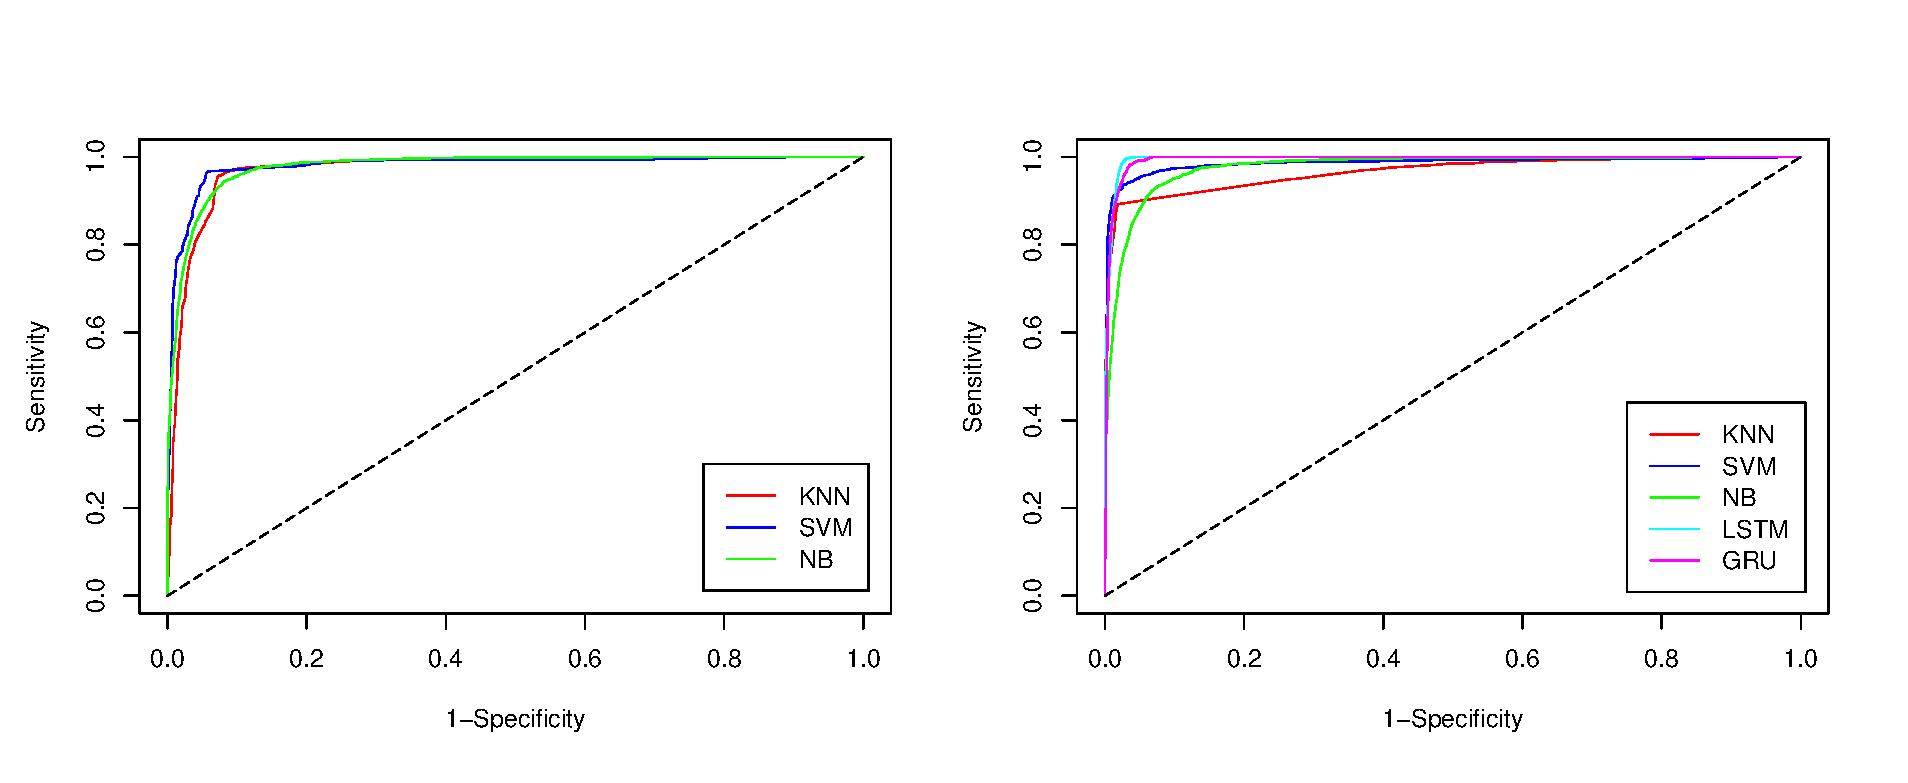
\includegraphics[width=1.0\textwidth]{figures/roc-curves.eps}
    \caption{\textbf{Receiver operating characteristic curves showing the performance of binary classifiers for the segmentation of e-Coaching text when lexical features (left) and combination of lexical, DL-LDA-based topic (except LSTM and GRU) and punctuation features (right) are used}.}
    \label{fig:roc-curves}
\end{figure}

% Baseline ROC results: BRNN: 0.9198, MLP: 0.9507, CRF: 0.9662, CRNN: 0.9648
% Proposed ROC Results: BRNN: 0.9807, MLP: 0.992, CRF: 0.9937, CRNN: 0.9859

In this paper, results are reported by each class to avoid confusion regarding overall model performance due to severe class imbalance. In addition, standard metrics: precision, recall and F1-measure were used to eliminate doubt about the model performance since accuracy is misleading for imbalanced datasets. AUC is also utilized due to its effectiveness in measuring the quality of binary classifiers for imbalanced datasets\cite{hu2015kernelized}, which are demonstrated by the ROC curves in Figure~\ref{fig:roc-curves}. Although NB provides lowest classification results, it shows moderate AUC values, achieving 0.978 AUC when only lexical features are used and 0.977 AUC when a combination of lexical, punctuation and topic features are used. On the other hand, KNN and SVM exhibit 0.972 and 0.986 AUCs when only lexical features are used; and 0.966 and 0.980 AUCs when a combination of lexical, punctuation and topic model-based features are used. Finally, LSTM demonstrates the highest AUC value among all machine learning models, achieving 0.996 AUC, while GRU achieves only 0.2\% lower AUC than LSTM.   

\begin{figure}[!htb]
    \centering
    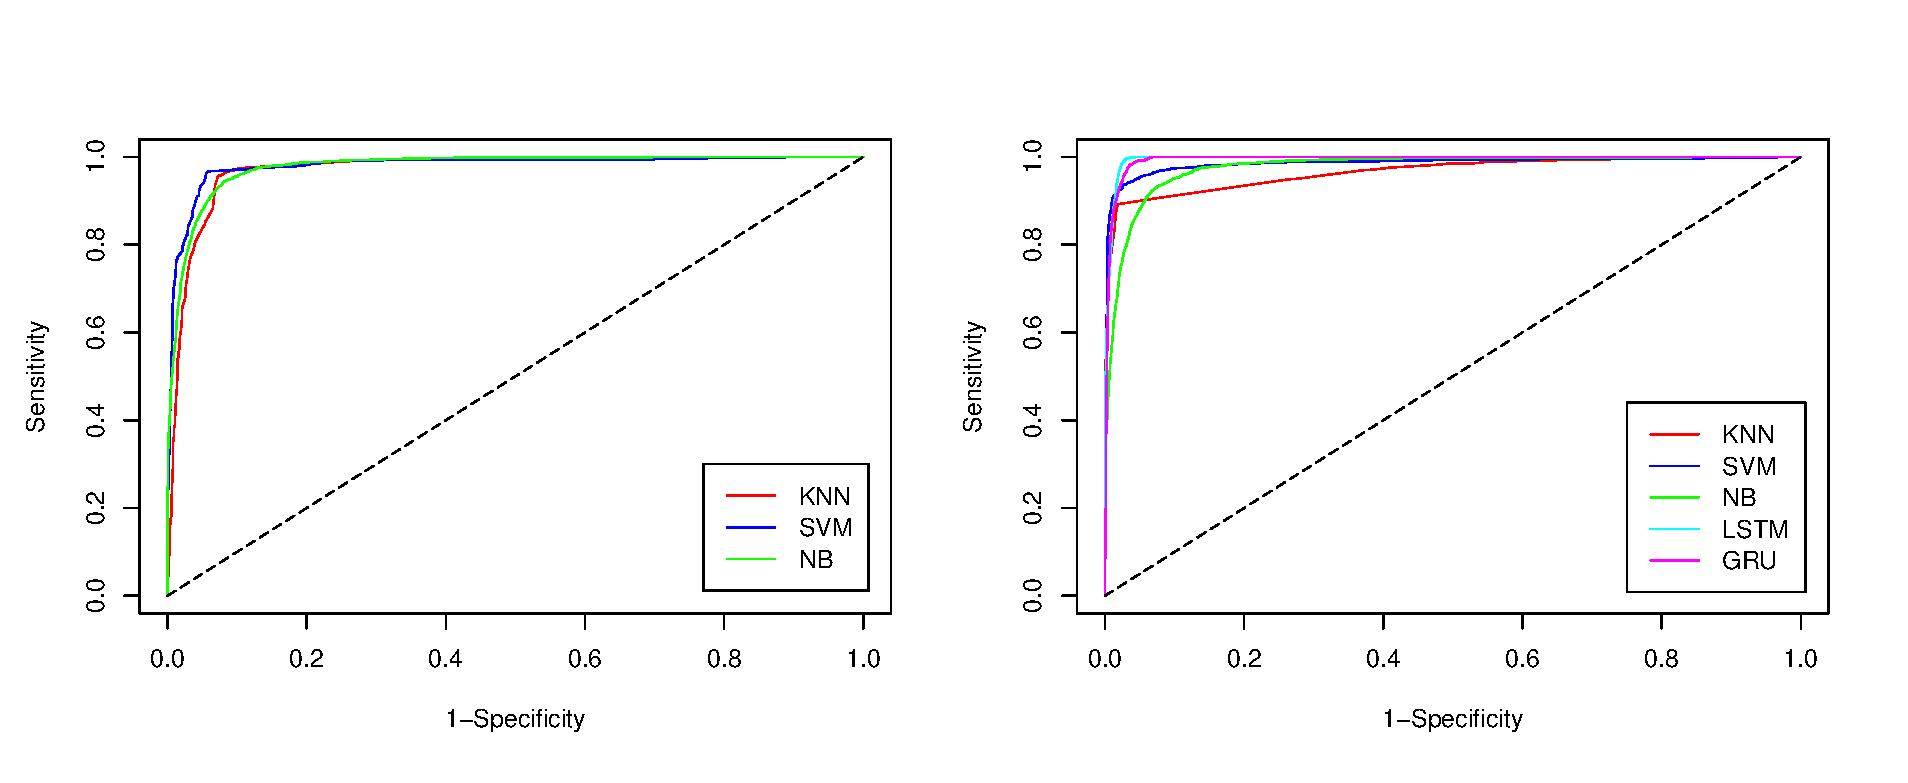
\includegraphics[width=1.0\textwidth]{figures/roc-curves.eps}
    \caption{\textbf{Receiver operating characteristic curves showing the performance of binary classifiers for the segmentation of e-Coaching text when lexical features (left) and combination of lexical, DL-LDA-based topic (except LSTM and GRU) and punctuation features (right) are used}.}
    \label{fig:roc-curves22}
\end{figure}   

We observed moderate performance of RNN, in particular, LSTM and GRU for the text segmentation. We believe that RNN will perform better if a larger dataset is utilized. In this study, we employed 3,138 examples of boundary case which limit to achieve the best performance. We also observed that GRU performs better than LSTM, which was observed in previous studies\cite{chung2014empirical}.

Although punctuation mark plays an important role in segmentation boundary detection and large numbers of errors were encountered by the false positive of boundary identification. For example, a text segment from an e-Coaching email \textit{``A typical day in regards to fruit and vegetable has me eating about a serving at breakfast (our caf has cut up fruit) and then maybe a piece of fruit later in the day or as a snack. Vegetable tends to be a side serving at lunch and dinner and I get celery or carrot cuts with dressing for a snack a lot of times. I could probably add some sort of vegetable into my breakfast (like spinach in an omelet) and snack on another piece of fruit when I quotemark m hungry rather than the junk food I tend to eat.''} incorrectly segmented after the first sentence where a punctuation mark was encountered. Similarly, additional information is a common cause for misclassification of an email segment into multiple segments. For instance, the first sentence of the above email segment represents a positive commitment to adolescent's behavior change then next two sentences provide an additional information to support their commitment. 

Our proposed approach is novel for the segmentation of e-Coaching emails since previous studies mainly focused on the segmentation of text into sections, headers and sentences. However, this study segmented clinical exchange into groups of MI behaviors which will significantly reduce the amount of resource and time required to segment clinical exchange manually. Furthermore, these segmentation models could be integrated with auto coding classifiers to build a software pipeline for automated annotation of exchanges.

The limitation of this study is that e-Coaching data is collected from a single medical institute; formatting, style and email segment can be different in other settings. Therefore, there is a need to replicate the experiments with different data sets. As our future work, we plan to evaluate our approach to other datasets for discourse analysis. 
 
\section*{Conclusion}
Segmentation of e-Coaching emails is an integral part of developing e-Coaching interventions. Although several studies have focused on clinical interventions, they are limited by the qualitative coding of clinical interactions. In addition, previous studies in the medical domain mainly segmented clinical text into sections and sentences, none of them considered segmentation of text into groups of MI behaviors in the setting of discourse analysis with emails. In this paper, we compared the performance of machine learning models for the task of segmentation of e-Coaching text. We found out that CRNN provides the best performance for the segmentation of text in terms of all performance metrics. Manual segmentation of e-Coaching data is very resource-intensive and time-consuming task, which can significantly decrease the time and effort required to develop an effective behavioral intervention. Our proposed methods can help to identify individual text segments, which can be annotated directly with a classification model. This approach will also help for developing fully automated e-Coaching and accelerate the pace of identifying effective communication strategies.

\section*{Acknowledgments}
This study was supported by a grant from the National Institutes of Health, NIDDK R21DK108071, Carcone and Kotov, MPIs. We would like to thank research staff and student assistants in the Department of Family Medicine and Public Health Sciences at Wayne State University School of Medicine for their help in preparing the training dataset. 

\bibliographystyle{vancouver}
\bibliography{manuscript}

\end{document}
